%%%%%%%%%%%%%%%%%%%%%%%%%%%%%%%%%%%%%%%%%
% Short Sectioned Assignment
% LaTeX Template
% Version 1.0 (5/5/12)
%
% This template has been downloaded from:
% http://www.LaTeXTemplates.com
%
% Original author:
% Frits Wenneker (http://www.howtotex.com)
%
% License:
% CC BY-NC-SA 3.0 (http://creativecommons.org/licenses/by-nc-sa/3.0/)
%
%%%%%%%%%%%%%%%%%%%%%%%%%%%%%%%%%%%%%%%%%

%----------------------------------------------------------------------------------------
%	PACKAGES AND OTHER DOCUMENT CONFIGURATIONS
%----------------------------------------------------------------------------------------

\documentclass[12pt,a4paper]{report}

\usepackage[T1]{fontenc} % Use 8-bit encoding that has 256 glyphs
\usepackage{fourier} % Use the Adobe Utopia font for the document - comment this line to return to the LaTeX default
\usepackage[english]{babel} % English language/hyphenation
\usepackage{amsmath,amsfonts,amsthm} % Math packages

\usepackage{lipsum} % Used for inserting dummy 'Lorem ipsum' text into the template

\usepackage{sectsty} % Allows customizing section commands
\allsectionsfont{\centering \normalfont\scshape} % Make all sections centered, the default font and small caps

\usepackage{fancyhdr} % Custom headers and footers

% use for graph
\usepackage{graphicx} 
\usepackage{subfigure}
\usepackage{caption}
\usepackage{float} 
\usepackage{url}
\usepackage[colorlinks,linkcolor=blue]{hyperref}
\usepackage{svg}
\usepackage{indentfirst} %每段的首行缩进
\hypersetup{
    colorlinks=true,
    linkcolor=blue, % 设置链接颜色为蓝色
    urlcolor=blue, % 设置网址颜色为蓝色
    citecolor=black
}

\usepackage{url}
\usepackage{graphicx}
\usepackage{listings}
\usepackage{xcolor}
\usepackage{amsmath}



\setlength{\abovecaptionskip}{10pt} % 设置图注上方的间隔为5pt
\setlength{\belowcaptionskip}{10pt} % 设置图注下方的间隔为-10pt


\begin{document}
% \maketitle % Print the title


\begin{titlepage} \vspace{1cm}

    \begin{center}
    \textbf{\Huge Modelling Biological Neural Networks}
    \end{center}
    
    \vspace{1.5cm}
    
    \begin{center}
    \textbf{\LARGE Ananthakrishnan Sumedan \\ Kai Deng \\ Laurel Dsouza }{\LARGE\par}
    \end{center}
    
    \vfill{}
    
    \begin{center}
    {\Large AM3064/AM6015 Written Report}
    \par\end{center}
    
    \vspace{1cm}
    
    \begin{center}
    \Large{School of Mathematical Sciences \\
    University College Cork \\
    Ireland \\
    6 April 2024}
    \end{center}
    
\end{titlepage}

This report is wholly the work of the author, except where explicitly
stated otherwise. The source of any material which was not created
by the author has been clearly cited. \\
\medskip{}

Date: 6 April

\medskip{}

Signature: Ananthakrishnan Sumedan, Kai Deng, Laurel Dsouza


\tableofcontents{}

\chapter{Author Contribution}



\begin{enumerate}
    \item[] \textbf{Ananthakrishnan Sumedan}
    \begin{enumerate}
        \item Part 4 Dynamics Of Neuron.   
    \end{enumerate}
\end{enumerate}


\begin{enumerate}
    \item[] \textbf{Kai Deng}
    \begin{enumerate}
        \item Part 1 Background Concept. 
        \item Part 2 Modelling History.
        \item Part 6 Applications.
        \item Initiated the GitHub repository for team coorporation.
        \item Initiated local VSCode LaTeX environment and shared how to configure it via Zoom meeting.
        \item Find a suitable PPT template for team and check the slides.
        \item Merge the report.
    \end{enumerate}
\end{enumerate}

\begin{enumerate}
    \item[] \textbf{Laurel Dsouza}
    \begin{enumerate}
        \item Part 3 Hodgkin-Huxley Model.
        \item Part 6 Code Python Implementation.
    \end{enumerate}
\end{enumerate}




\clearpage

\chapter{Background Concept}
\section{Anatomy of a Neuron}
Neurons are cells — small bodies of mostly water, ions, amino acids and proteins with remarkable electrochemical properties. They are the primary functional units of the brain. Our mental experiences — our perceptions, memories, and thoughts — are the result of the ebb and flow of salts across neural bi-lipid membranes and the synaptic transmissions between neurons. 

Neurons receive signals from other neurons through synapses located – not exclusively – on their dendritic tree, which is a complex, branching, sprawling structure. If you are wondering what the king of dendritic complexity is, that would be the Purkinje cell, which may receive up to 100,000 other connections. Dendrites are studded with dendritic spines – little bumps where other neurons make contact with the dendrite.

\vspace{10pt}
Signals from the dendrites propagate to and converge at the soma – the cell’s body where nucleus and other typical cell organelles live.

\vspace{10pt}
Coming off the soma is the axon hillock which turns into the axon. The axon meets other neurons at synapses. It allows a neuron to communicate rapidly over long distances without losing signal integrity. To allow signals to travel rapidly, the axon is myelinated – it is covered with interspersed insulators which allows the neuron’s signal to jump between insulated sections. To allow the signal to maintain integrity, the neuron signal in the axon is ‘all-or-nothing’ – it is a rather bit-like impulse, which we will discuss next.


\begin{figure}[H]
    \centering
    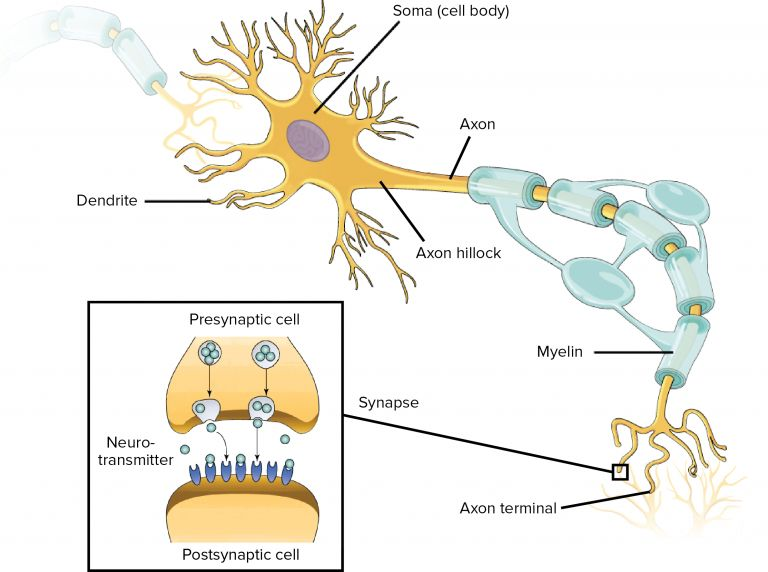
\includegraphics[width=0.7\textwidth]{./data/neural.jpg}
    \caption{Anatomy of the neuron}
    \label{fig:my_picture}
    \vspace{1pt} % Vertical space, optional
    \small{Source: Source:“Neurons and glial cells” by OpenStax College, Biology CC BY-NC-SA 3.0 License.}
\end{figure}


\section{Physiology of a Neuron}

The second thing to appreciate about neurons is their specialized physiology — that is the cellular functions of neurons. The most striking feature of neural cellular function is the action potential. This is the mechanism which allows neurons to transmit information reliably over long distances without the transmission attenuating.

\vspace{10pt}
It is important to remember that neurons bathe in an extracellular solution of mostly water, salts and proteins. The forces caused by the movement of salts into and out of the cell and the different concentrations of these salts is the physical basis of the neuron’s remarkable behavior. There are sodium-potassium pumps which move sodium out of the cell and potassium in, so that the concentration of sodium outside the cell is higher than inside and the concentration of potassium outside the cell is lower then inside.

\vspace{10pt}
An action potential is a discrete event in which the membrane potential rapidly rises (depolarizes) and then falls (polarizes). This discrete event is all-or-nothing, meaning that if an action potential occurs at one part of the neurons membrane, it will also occur in the neighboring part, and so on until it reaches the axon terminal. Action potentials do not tend to travel backwards, because, once a section of the membrane has fired an action potential, electrochemical-forces hyper-polarize the region of membrane while the channels which were previously open close and become inactive for some duration of time.

\vspace{10pt}
The action potential is the result of different species of ions traveling across the cell membrane through channels and the activation and inactivation of those channels on different time scales. A stereotypical action potential occurs as follows:

\begin{figure}[H]
    \centering
    \begin{minipage}[b]{0.45\textwidth}
      \centering
      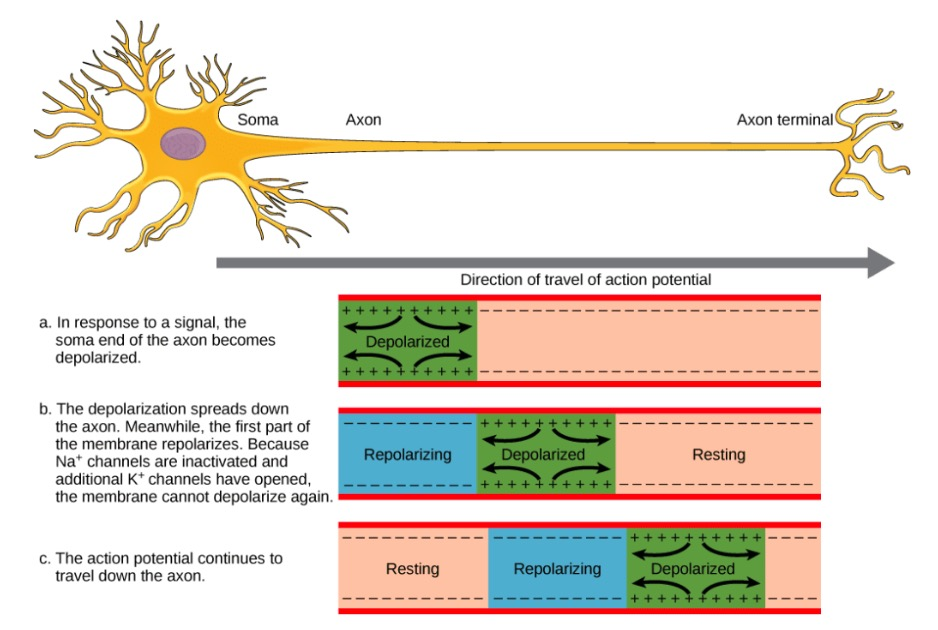
\includegraphics[width=\textwidth]{./data/propagation-of-nerve-impluse.jpg}
      \caption{Propagation of nerve impluse}
      \label{fig:exampleA}
      \vspace{1pt} % Vertical space, optional
      \small{Source: \href{https://opentextbc.ca/biology/chapter/16-2-how-neurons-communicate/}{Opentex}}
    \end{minipage}
    \hfill
    \begin{minipage}[b]{0.45\textwidth}
      \centering
      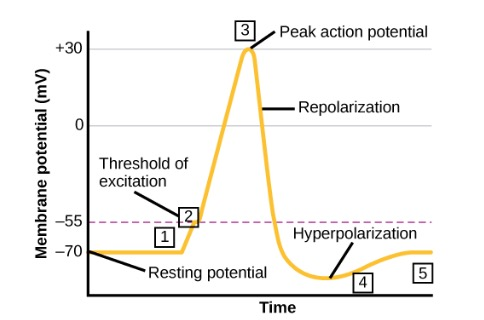
\includegraphics[width=\textwidth]{./data/neuronal-action-potential.jpg}
      \caption{Neuronal action potential}
      \label{fig:exampleB}
      \vspace{1pt} % Vertical space, optional
      \small{Source: \href{https://opentextbc.ca/biology/chapter/16-2-how-neurons-communicate/}{Opentex}}
    \end{minipage}
\end{figure}

\begin{itemize}
    \item \textbf{Equilibrium:} The neuron’s equilibrium membrane potential is near \(-70\) mV — roughly the Nernst Equilibrium of \( E_{K^+} \approx -75 \). At equilibrium, the net current is \(0\) — inward and outward currents are balanced.
    \item \textbf{Depolarization:} Incoming excitatory signals depolarize the membrane. Quick-to-respond voltage gated \( Na^+ \) channels are activated, and \( Na^+ \) rushes in, pushing the membrane potential higher. Slower-to-respond \( K^+ \) channels open, and \( K^+ \) rushes out, pushing the membrane potential lower.
    \item \textbf{Amplification:} If the neuron becomes more stimulated or is stimulated rapidly, many more \( Na^+ \) channels are activated than \( K^+ \) channels. This causes a feedback loop where the influx of \( Na^+ \) causes more \( Na^+ \) channels to activate.
    \item \textbf{Repolarization:} Eventually the membrane potential is near the Nernst Equilibrium of \( Na^+ \) as the sodium channels are maximally open. The slower \( K^+ \) channels catch up to \( Na^+ \), which repolarizes the membrane potential. Meanwhile, the \( Na^+ \) channels become inactive.
    \item \textbf{Hyper-polarization:} \( K^+ \) channels are open while \( Na^+ \) channels are inactive, causing the membrane potential to dip below its typical equilibrium point, near the \( K^+ \) Nernst equilibrium.
    \item \textbf{Refractory Period:} The \( Na^+ \) channels, take a while to become deinactivated, meaning after an action potential, they remain incapable of opening again for a period of time. The period in which most \( Na^+ \) channels are called the absolute refractory period (the neuron cannot spike no matter the strength of the stimulus) while the period in which many \( Na^+ \) channels are inactivated is called the relative refractory period (the neuron can spike given a sufficiently strong stimulus).
\end{itemize}



\section{Spike train}

Spike trains are the language of neurons. People tend to think of spikes as point-events and spike trains as point-processe. We describe these with the neural response function:

\begin{equation}
    \rho(t) = \sum_{i=1}^{k} \delta(t-t_i)
\end{equation}

where an impulse is defined as the dirac delta function (which is convenient for counting things):

\begin{equation}
    \delta(t) = \begin{cases} 1 & \text{if } t = 0, \\ 0 & \text{otherwise} \end{cases}
\end{equation}

Often, it is useful for analysis to assume spike trains are generated by random processes. Assuming spikes are independent of each other, we can model this point process is a Poisson process, in which we know the probability n spikes occur in the interval $\Delta T$:

\begin{equation}
    P\{n \text{ spikes occur in } \Delta t\} = \frac{(rt)^n}{n!} \exp(-rt)
\end{equation}

To generate spikes according to a Poisson point process, generate a random number r in a sufficiently small time interval, such that only 1 spike should occur, and check whethe $r < firingRate \Delta T$. However, make sure that $firingRate\Delta T < 1$.

\section{Biological Neural Networks}
Biological neural networks are the complex systems of neurons and their connections in organisms, crucial for processing and transmitting information, enabling perception, decision-making, and behavior. Modeling these networks through computational frameworks aims to replicate their structure and function, shedding light on how information processing leads to complex cognitive functions and behaviors. 
Understanding neurons and neural computation can provide biological inspiration for new ways to process information and for artificial intelligence.


\chapter{Modelling History}

\section{The M-P model}
Since the Spanish anatomist Cajal founded the neuron theory at the end of the 19th century, the biological characteristics and related electrical properties of neurons have been discovered one after another. In 1943, the M-P model of neurons (shown in Figure 1.4) was first proposed in the paper "Logical Activities of Thoughts Contained in Neural Activities" \cite{Mcculloch1854LOGICALCALCULUSIDEAS}. The model was created by psychologists W.S. McCulloch and W.S. McCulloch from the United States. Another mathematician, W.A. Pitts.

\begin{figure}[H]
    \centering
    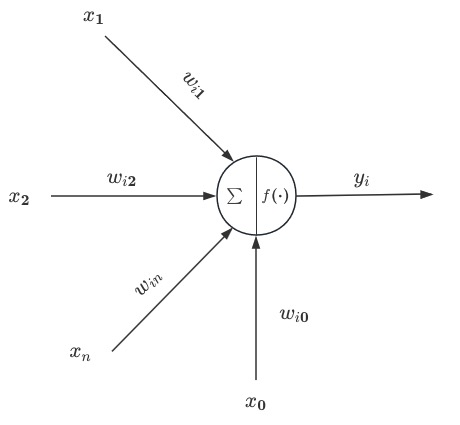
\includegraphics[width=0.9\textwidth]{./data/M-P.jpg}
    \caption{Schematic diagram of the M-P model of neurons}
    \label{fig:my_picture}
    \vspace{1pt} % Vertical space, optional
\end{figure}

In the figure, $x_i$, 1, 2, ..., represents the input signal transmitted from other neurons connected to the current neuron, $w_{ij}$ represents the connection strength or weight from neuron j to neuron i, $\theta_i$ is the neuron The activation threshold or bias of the element, f is called the activation function or transfer function. The output of the neuron $y_i$ can be expressed as follows:

\begin{equation}
    y_i = f(\sum_{j=i}^{n} w_{ij}x_j-\theta_i)
\end{equation}

This model describes neurons from the perspective of logical functional devices, opening up a path for theoretical research on neural networks. The M-P model is a mathematical simplification of the biological neuron information processing model, and subsequent neural network research work is based on it. 

The Mp model gets inspiration from threshold theory in nerve impulses and Applies it in logical neurons and it builds a groundwork for the development of more complex activation functions used in neural networks today.



\section{Hebb learning rules}
In 1949, in the book "The Organization of Behavior", the psychologist Donald O. Hebb analyzed the change rules of the connection strength between neurons, and based on this, he proposed the famous Hebb learning rule \cite{Hebb2002OrganizationBehaviorNeuropsychological}. Inspired by Pavlov's conditioned reflex experiments, Hebb believed that if two neurons are fired at the same moment, the connection between them should be strengthened. The Hebb learning rule defined based on this is as follows:

\begin{equation}
    w_{ij}(t + 1) = w_{ij}(t) + \alpha y_j(t)y_i
\end{equation}

Among them, $w_{ij}(t+1)$ and $w_{ij}(t)$ represent the connection strength between neuron j and neuron i at time t and t + 1 respectively, while $y_i$ and $y_j$ are the outputs of neurons i and j.


Hebb's rule belongs to the category of unsupervised learning algorithms. Its main idea is to adjust the connection relationship between two neurons according to their excitation state, so as to realize the simulation of simple neural activities. Following the Hebb learning rule, the supervised delta learning rule of neurons was proposed to solve the learning problem of neuron weights when the input and output are known. This algorithm continuously adjusts the connection weights to make the actual output of the neuron consistent with the expected output. Its learning correction formula is as follows


\begin{equation}
    w_{ij}(t + 1) = w_{ij}(t) + \alpha(d_i - y_i)x_j(t)
\end{equation}

Among them, $\alpha$ is the learning rate of the algorithm, $d_i$ and $y_i$ are the expected output and actual output of neuron i, $x_j{t}$represents the state (activation or inhibition) of neuron j at time t.

Intuitively speaking, when the actual output of neuron i is greater than the expected output, the connection weight with the activated neuron is reduced, and the connection weight with the inhibited neuron is increased; when the actual output of neuron i is greater than the expected output If it is small, the connection weight with activated neurons will be increased, while the connection weight with inhibited neurons will be reduced. Through such an adjustment process, neurons will store the correct mapping relationship between input and output in the weight, thus possessing the ability to represent data. The Hebb learning rule and the Delta learning rule are both proposed for a single neuron. The learning rules for parameters in a network composed of neurons will be discussed later. The research work done by the above pioneers paved the way for the emergence of neural computing and inspired many scholars to continue exploring and researching this field.


\section{Delta learning rules}

The basic idea of the delta learning rule is to reduce the difference between the network output and the target output by continuously adjusting the network weights. It determines the adjustment direction and size of the weight by calculating the gradient of the error. At each iteration, the weights are adjusted slightly in the opposite direction of the gradient to gradually reduce the error.
A common delta learning rule is a variant of the delta rule, called the delta rule or Widrow-Hoff rule \cite{BernardWidrow1960AdaptiveSwitchingCircuits}. This rule is based on the perceptron model and updates the weights based on the difference between the actual output and the desired output. The size of the update depends on the size of the input signal as well as the error signal.

The Delta learning rule, also known as the Widrow-Hoff rule, is a simple algorithm used for adjusting the weights of connections in a neural network during training. The formula for updating the weights in the Delta learning rule is as follows:

\[ \Delta w_{ij} = \eta \cdot (d_j - y_j) \cdot x_i \]

Where:

\begin{itemize}
    \item \textbf{ $\Delta w_{ij}$:} is the change in weight between neuron \( i \) and neuron \( j \).
    \item \textbf{$\eta $:} is the learning rate, which controls the step size of the weight update.
    \item \textbf{ $d_{j}$:} is the target output for neuron \( j \).
    \item \textbf{$y_j$:} is the actual output of neuron \( j \).
    \item \textbf{$x_i$:} is the input from neuron \( i \) to neuron \( j \).
\end{itemize}

This formula calculates the change in weight \( \Delta w_{ij} \) based on the error between the target output \( d_j \) and the actual output \( y_j \), multiplied by the input \( x_i \) and the learning rate \( \eta \). The weight update is applied to all connections in the network during each training iteration.


Delta learning rules are widely used in neural network training, especially in supervised learning tasks such as classification and regression. It provides an effective method for neural networks to automatically adjust weights to gradually improve the performance and accuracy of the network.

Both Hebb learning rules and Delta learning rules provide a certain foundation and inspiration for the development of backpropagation algorithm.



\section{Mark I perceptron}

In 1958, F. Rosenblatt invented the perceptron model (Perceptron), which was the first model in history to introduce the concept of neural networks into electronic computer processing, marking a new stage in the development of neural networks \cite{Rosenblatt1958PerceptronProbabilisticModel}. The perceptron is a binary linear classification model that determines the output of a two-class model by weighted summation of the input features followed by an activation function. The activation function is a step function, used to determine whether the input value is positive or negative. The mathematical representation of the perceptron model is as follows, where \( x \) represents the input vector, \( w \) represents the weight vector, \( b \) represents the bias term, and \( y \) is the output value, which can be \(+1\) or \(-1\), with the mathematical representation being:

\begin{equation}
    y = f(x) = \text{sign}(w \cdot x + b)
\end{equation}

Here, \( w \cdot x \) represents the dot product of vectors \( w \) and \( x \), and the definition of the \( \text{sign} \) function is as follows:

\begin{equation}
    \text{sign}(x) = 
\begin{cases}
+1, & \text{if } x \geq 0 \\
-1, & \text{if } x < 0
\end{cases}
\end{equation}


The perceptron learning algorithm is based on the principle of reducing the error of classification. When the classification result is incorrect, it adjusts the weights and biases, thus improving the classification ability step by step. The perceptron learning algorithm aims to find the weights and biases that minimize the classification error. Let's define a training set \( T = \{(x_1, y_1), (x_2, y_2), \ldots, (x_n, y_n)\} \), where \( x_i \) is the input vector and \( y_i \) is the corresponding output. The goal of the perceptron learning algorithm is to minimize the loss function \( L(w,b) \):

\begin{equation}
L(w,b) = - \sum_{x_i \in M} y_i (w \cdot x_i + b)
\end{equation}

where \( M \) is the set of misclassified examples. The perceptron updates the weights \( w \) and bias \( b \) to minimize \( L(w,b) \):

\begin{equation}
\min_{w,b} L(w,b) = - \sum_{x_i \in M} y_i (w \cdot x_i + b)
\end{equation}

The gradient descent method is used to update the weights and biases, which aims to adjust the weights and biases in the opposite direction of the gradient of the loss function. The updates for weights \( w \) and bias \( b \) are as follows:

\begin{equation}
\nabla_w L(w,b) = - \sum_{x_i \in M} x_i \cdot y_i
\end{equation}

\begin{equation}
\nabla_b L(w,b) = - \sum_{x_i \in M} y_i
\end{equation}

Therefore, each time an example \( (x_i, y_i) \) is misclassified, the weights \( w \) and bias \( b \) are updated as follows:

\begin{equation}
w_{\text{new}} = w_{\text{old}} + \eta y_i x_i
\end{equation}

\begin{equation}
b_{\text{new}} = b_{\text{old}} + \eta y_i
\end{equation}

where \( \eta \) is the learning rate, a positive constant determining the size of the update step.


In the algorithm, \( 0 < \eta \leq 1 \) is the learning rate. It determines the size of the adjustment to the weights during the learning process. When the perceptron classifies an example correctly, the weights and bias are not adjusted. When it misclassifies an example, it adjusts the weights and bias towards the direction that could possibly correct the error. This process is not changed until all examples are classified correctly, or the process reaches a preset number of iterations. According to the update rules from equations (10) and (11), the weights \( w \) and bias \( b \) are adjusted as follows:

\begin{equation}
w = \sum_{i=1}^{n} a_i y_i x_i
\end{equation}

\begin{equation}
b = \sum_{i=1}^{n} a_i y_i
\end{equation}

where \( a_i = \eta n_i \), and \( n_i \) is the number of times the perceptron misclassified the \( i \)-th example. The perceptron algorithm is named after the psychologist Frank Rosenblatt, who, along with engineers B. Widrow and M. Hoff, adapted the ADALINE (ADAptive LINear Element) from the model of the same name developed by H. Steinbuch.


\section{Hopfield neural network model}
The next significant advancement in the field of neural networks occurred in 1969 when M. Minsky and S \cite{JJHopfield1982NeuralNetworksPhysical}. Papert pointed out the limitations of the perceptron in their book "Perceptrons," demonstrating that it was incapable of processing the XOR problem. However, this criticism also motivated further research into neural networks with additional layers, leading to the development of multilayer networks. The key breakthrough was the introduction of the "backpropagation" algorithm that enabled the training of multilayer networks.

A single-layer perceptron can only solve problems linearly separable because it is essentially a linear classifier. It was realized that to overcome the limitations of the perceptron and solve non-linearly separable problems, one must utilize multilayer networks and non-linear activation functions. The first step in this direction was taken by introducing the concept of a neural network capable of associative memory, which led to the invention of the Hopfield network by J.J. Hopfield in 1982.

The Hopfield network, an energy-based model, is particularly known for solving the Travelling Salesman Problem (TSP). It opened new avenues for using neural networks in optimization problems beyond the domain of traditional computation.

Hopfield's work not only advanced the theoretical foundations of neural networks but also laid the groundwork for the development of modern neural networks, which are capable of learning complex patterns and solving diverse problems. This laid the foundation for significant strides in the field of neural networks, inspiring subsequent developments.

The Hopfield network is characterized by its feedback loops as shown in the figure. In the network, the output of each neuron is fed back into itself and other neurons through a set of resistors. Each neuron has a resistance \( R_i \) and a capacitance \( C_i \), and is connected to other neurons via resistors \( R_{ij} \) (where \( i,j = 1,2,...,n \); \( i \neq j \)). Each neuron's voltage \( U_i \) changes according to the charge \( Q_i \) and its voltage is fed back to itself through a resistor \( R_i \), and to other neurons through resistors \( R_{ij} \), (\( i,j = 1,2,...,n \)) with different resistances. The network follows Kirchhoff's Current Law (KCL), and the voltage change at each neuron is described by the following equation:

\begin{equation}
    \sum_{j=1}^{n} \frac{V_j(t)}{R_j} + I_i = C_i \frac{dU_i(t)}{dt} + \frac{U_i(t)}{R_i}, \quad i = 1, 2, \ldots, n
\end{equation}

However, in a Hopfield network, each neuron's voltage is modified by an activation function \( f \) to produce an output \( V_i \):

\begin{equation}
    V_i(t) = f_i(U_i(t)), \quad i = 1, 2, \ldots
\end{equation}

Then, the state energy of a Hopfield network is defined as:

\begin{equation}
W = R_{i,j}^{-1} (i,j=1,2,...,n)
\end{equation}

where \( R_i' \) are the weights of the network. The energy function of the Hopfield network is given by:

\begin{equation}
    E(t) = -\frac{1}{2} \sum_{i=1}^{n} \sum_{j=1}^{n} \frac{V_i(t)V_j(t)}{R_{ij}} - \sum_{i=1}^{n} V_i(t)I_i + \sum_{i=1}^{n} \frac{1}{R_i} \int_{0}^{V_i(t)} f^{-1}(V) \, dV
\end{equation}

Finally, a Hopfield network adjusts its state iteratively to minimize the energy function \( E(U) \), which leads to stable states—these are the solutions to the problem that the network is trying to solve. The dynamics of a Hopfield network's voltage adjustment towards stable states is analogous to the process of a physical system reaching its lowest energy state.

The Hopfield network is a recurrent neural network, which is to say, it possesses feedback loops. This feature allows it to have dynamic memory. Dynamic memory is different from the static memory seen in the perceptron, which only allows for the storage of a fixed set of patterns. The Hopfield network can store a variety of patterns and retrieve them based on the input, making it a form of associative memory.

Hopfield's paper not only triggered the renaissance of interest in neural networks but also led to the exploration of new types of neural networks. One significant development in this area was the Boltzmann machine, introduced by G.E. Hinton, T.J. Sejnowski, and D.H. Ackley in 1983. This machine was an extension of the Hopfield network and could solve problems that Hopfield networks could not.


\chapter{Hodgkin-Huxley Model}

\section{Introduction}

The Hodgkin-Huxley model, proposed by Sir Alan Hodgkin and Sir Andrew Huxley in 1952, revolutionized the field of neuroscience by providing a quantitative understanding of the generation and propagation of action potentials in neurons. This mathematical framework emerged from a decade-long collaboration between Hodgkin and Huxley, culminating in the publication of their landmark papers in the Journal of Physiology.

\subsubsection{Historical Background}

The Hodgkin-Huxley theory emerged as a result of a remarkable collaboration between Hodgkin and Huxley from the late 1930s to the early 1950s. Their work was informed by several key experimental findings. Cole and Curtis demonstrated that the action potential is associated with a significant increase in membrane conductance, laying the groundwork for understanding neuronal excitability\cite{Cole1939}. Subsequently, Hodgkin and Huxley performed the first intracellular recording of an action potential, revealing that the membrane potential during an action potential exceeds zero mV, thereby challenging existing hypotheses\cite{Hodgkin1939}. This experimental breakthrough was complemented by the theoretical insights of Hodgkin and Katz, who explained the overshooting action potential by elucidating the role of sodium permeability\cite{Hodgkin1949}. Additionally, Hodgkin, Huxley, and Katz developed a voltage-clamp circuit, following the pioneering work of Cole and Marmont, enabling precise measurement of ionic currents in squid axons\cite{Hausser2000}.

\section{Biological Basis of Neuronal Excitability}

Neuronal excitability, the ability of neurons to generate and transmit electrical signals, is fundamental to their function in the nervous system. This excitability arises from the intricate interplay of ion channels and the dynamic changes in membrane potential they produce.

\subsection{Resting Membrane Potential}

The resting membrane potential of a neuron, typically ranging from -60 mV to -70 mV, is maintained by the selective permeability of the cell membrane to different ions. This selective permeability is primarily mediated by resting ion channels, particularly those permeable to potassium ions. At rest, these channels allow a small efflux of K+ ions, establishing the negative charge within the cell compared to the extracellular space.

\begin{figure}[htbp]
    \centering
    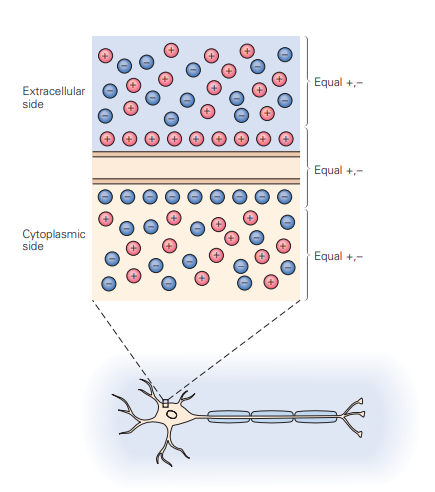
\includegraphics[width=0.6\textwidth]{./data/resting_membrane_potential.png}
    \caption{Resting membrane potential (Source: Principles of Neural Science\cite{principles_of_neural_science})}
    \label{fig:resting_membrane_potential}
\end{figure}

\subsection{Generation of Action Potentials}

Action potentials, the transient electrical signals responsible for rapid communication within the nervous system, are generated when the membrane potential depolarizes beyond a certain threshold. This depolarization is initiated by the opening of voltage-gated sodium channels in response to a stimulus. As Na+ ions rush into the cell, the membrane potential becomes more positive, reaching around +40 mV.

\subsection{Propagation of Action Potentials}

Once initiated, the action potential propagates along the axon of the neuron. This propagation occurs through a self-regenerating process where the depolarization of one region of the membrane triggers the opening of voltage-gated sodium channels in the adjacent region, leading to further depolarization. This continues along the length of the axon, allowing the action potential to travel rapidly towards the synapse.

\subsection{Repolarization and Hyperpolarization}

Following depolarization, the membrane potential undergoes repolarization, returning to its resting state. This repolarization is driven by the opening of voltage-gated potassium channels, allowing K+ ions to exit the cell, while voltage-gated sodium channels undergo inactivation. In some cases, repolarization may overshoot, leading to hyperpolarization, before eventually returning to the resting membrane potential\cite{principles_of_neural_science}.

\section{Formulation of the Hodgkin-Huxley Model}

The Hodgkin-Huxley model provides a quantitative description of membrane currents and their role in nerve conduction and excitation. Central to this model is the representation of the neuronal membrane as an electrical circuit, which captures the dynamics of ion flow across the membrane during the generation and propagation of action potentials.

\begin{figure}[htbp]
    \centering
    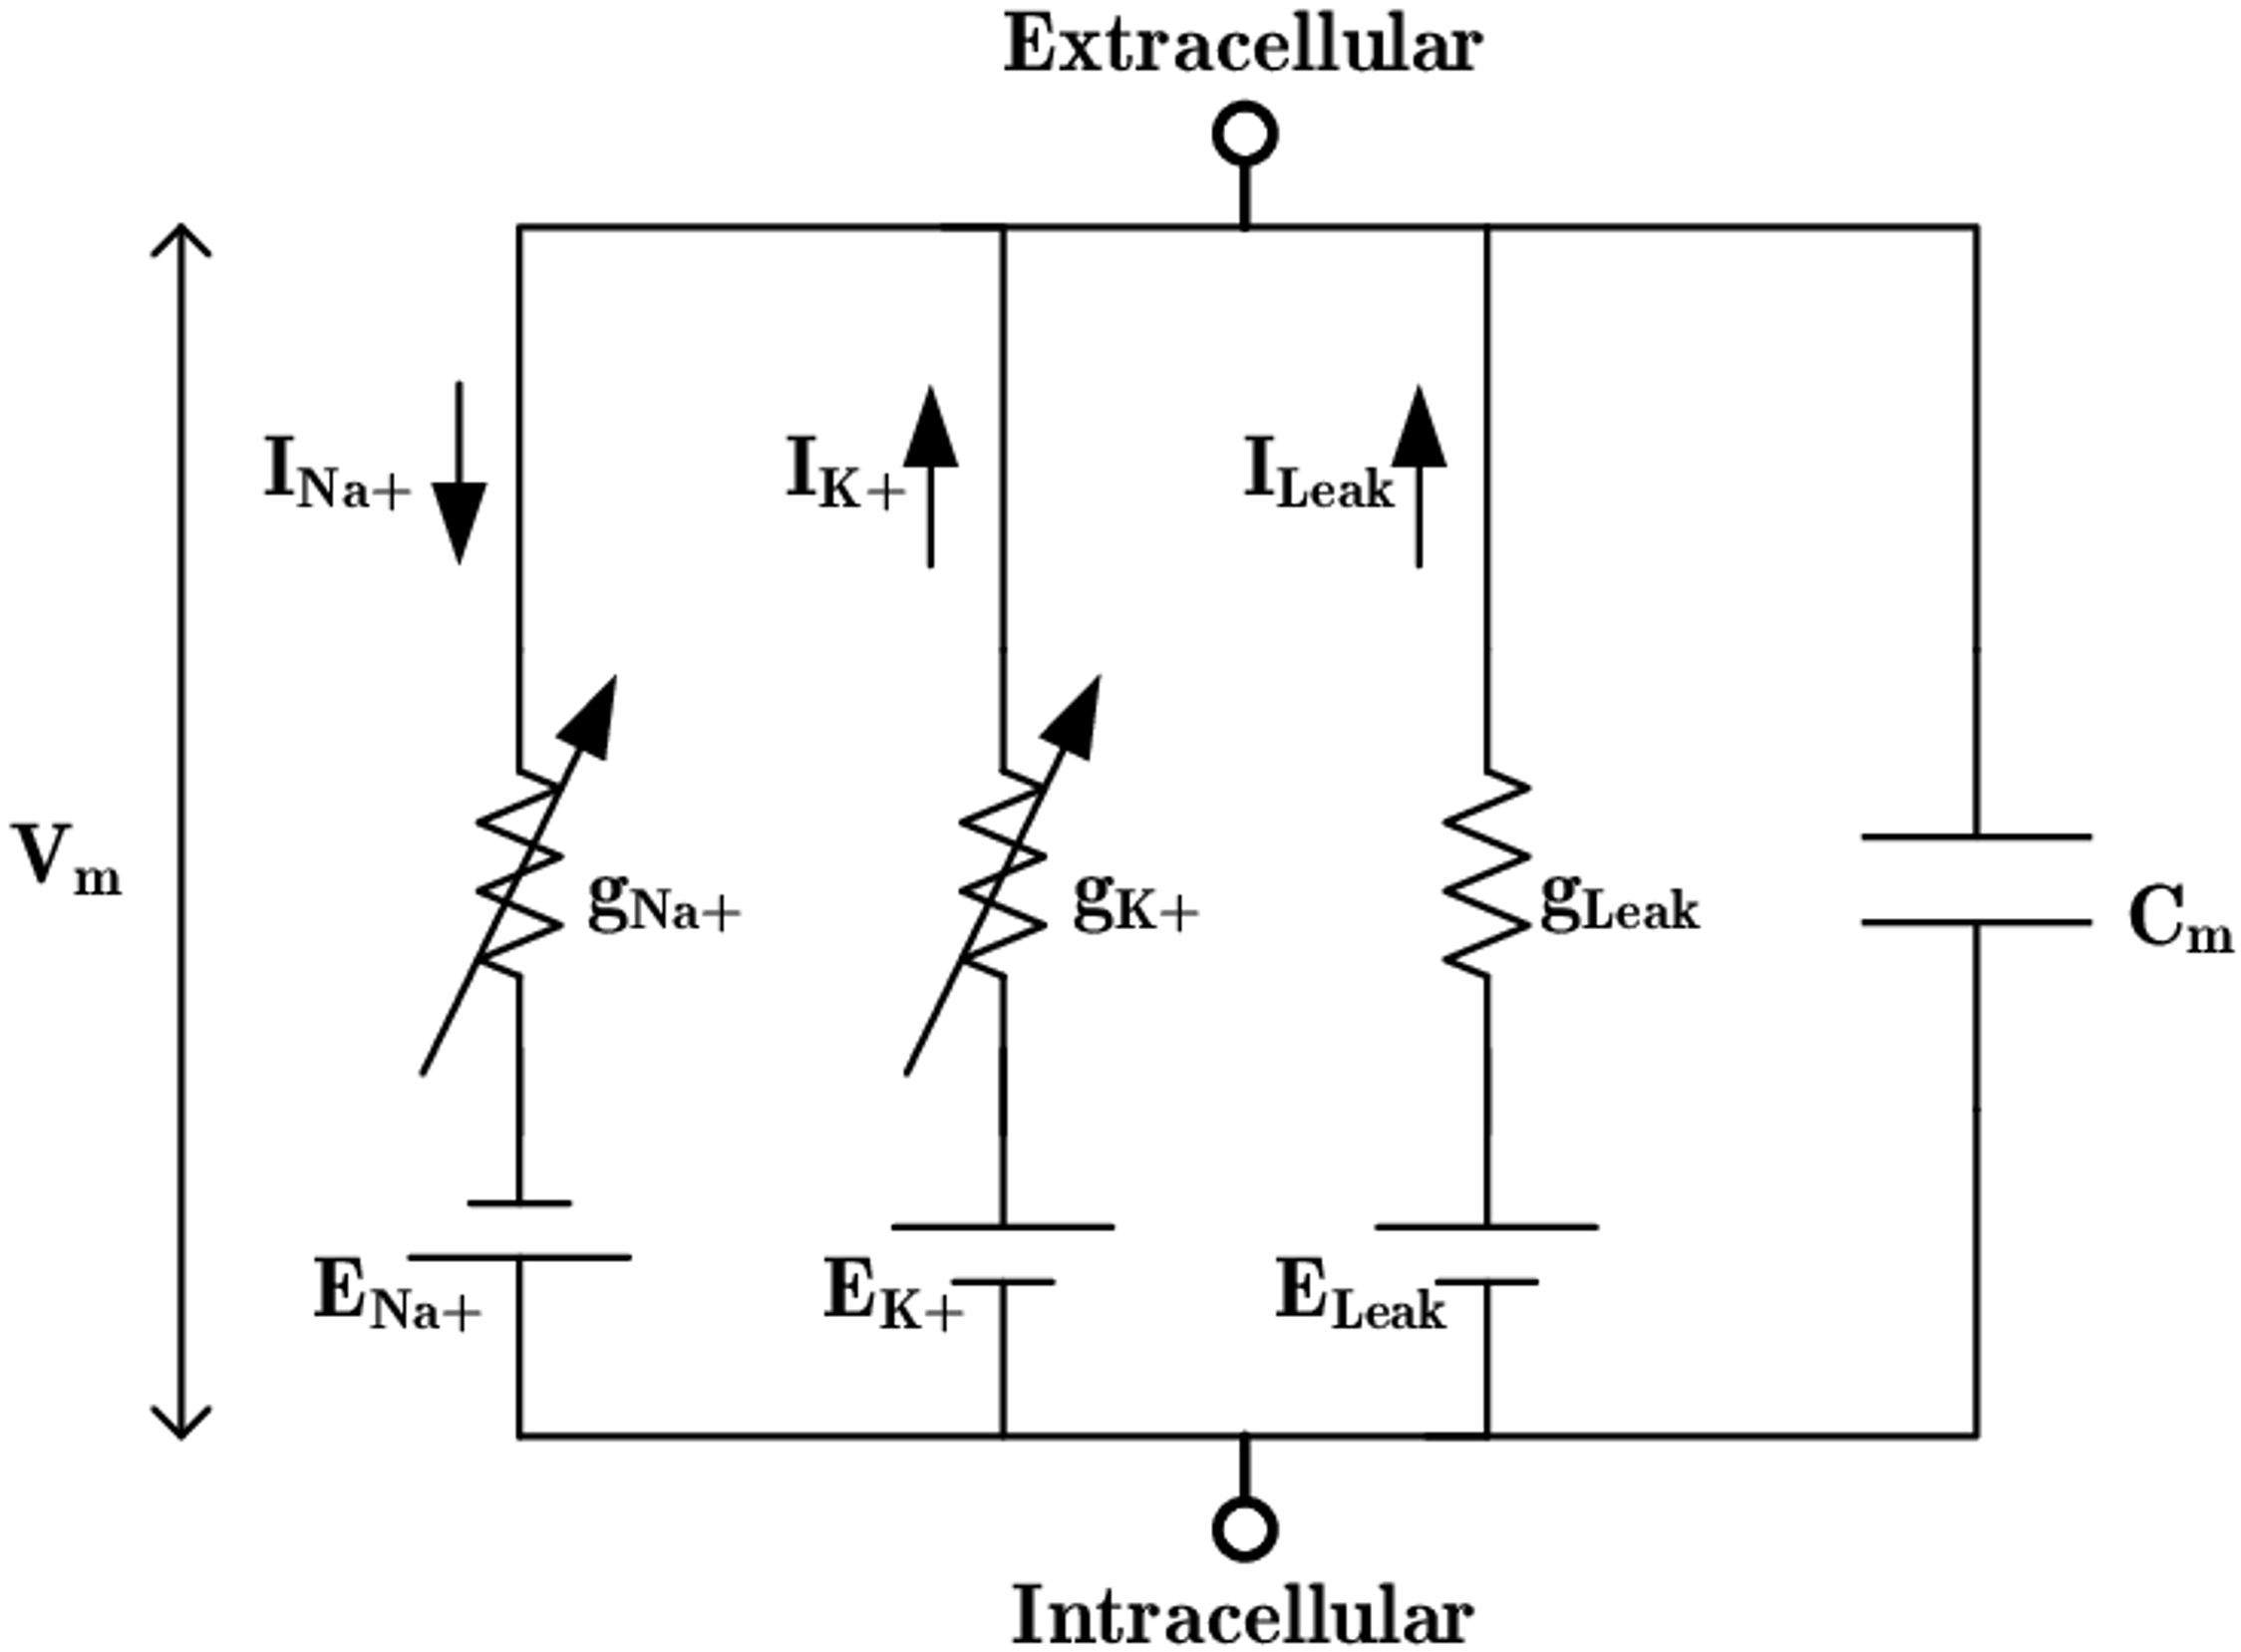
\includegraphics[width=0.6\textwidth]{./data/electrical_circuit_representing membrane.png}
    \caption{Electrical circuit representing membrane. (Source: A quantitative description of membrane current and its application to conduction and excitation in nerve\cite{Hodgkin1952})}
    \label{fig:electrical_circuit_representing membrane.}
\end{figure}

\subsection{Electrical Circuit Representation}

In the Hodgkin-Huxley model, the neuronal membrane is represented as an electrical circuit composed of several components.

Membrane Capacitance (C): The lipid bilayer of the neuronal membrane acts as a capacitor, storing charge and contributing to the membrane's ability to maintain a voltage gradient.

Ion Channels: Voltage-gated ion channels, including sodium (Na+), potassium (K+), and leak channels, are represented as resistors in the circuit. These channels control the flow of ions across the membrane in response to changes in membrane potential.

Battery (Em): The battery in the circuit represents the resting membrane potential, which is typically around -60 to -70 mV in neurons. It serves as the reference voltage against which changes in membrane potential are measured.

\subsection{The Hodgkin-Huxley Equation}

The Hodgkin-Huxley model provides a quantitative description of membrane current and its application to conduction and excitation in nerve cells. It represents the dynamic interplay of ion channels and membrane capacitance in generating and propagating action potentials.

The model is formulated based on the principles of electrical circuits. The total current in the neuron can be expressed as the sum of the individual ion currents and the capacitive current:
\[
I_{\text{Total}} = I_{\text{Na}} + I_{\text{K}} + I_{\text{leak}} + I_{\text{C}}
\]

Using the relationship between charge ($Q$), capacitance ($C$), and potential difference ($V$):
\[
C = \frac{Q}{V}
\]

We can express the capacitive current ($I_C$) as the rate of change of charge with respect to time:
\[
C \frac{dV}{dt} = I_{\text{Total}} - I_{\text{Na}} - I_{\text{K}} - I_{\text{leak}}
\]

Applying Ohm's law ($I = \frac{V}{R}$), where $R$ is the resistance, to each ion current:
\[
I = \frac{1}{R} \times V
\]

We can modify this to incorporate the reversal potential ($E$):
\[
I = \frac{1}{R} \times (V - E)
\]

Substituting these into the equation for the capacitive current:
\[
C \frac{dV}{dt} = I_{\text{Total}} - \frac{1}{R_{\text{Na}}} \times (V_m - E_{\text{Na}}) - \frac{1}{R_{\text{K}}} \times (V_m - E_{\text{K}}) - \frac{1}{R_{\text{leak}}} \times (V_m - E_{\text{leak}})
\]

Where $V_m$ represents the membrane potential, and $E_{\text{Na}}$, $E_{\text{K}}$, and $E_{\text{leak}}$ represent the equilibrium potentials for sodium, potassium, and leak currents respectively.

Expanding the equation using the Hodgkin-Huxley model for the conductance of each ion ($g$) and the gating variables ($m$, $h$, $n$):
\begin{align*}
C \frac{dV}{dt} & = I_{\text{Total}} - g_{\text{Na}} m^3 h (V_m - E_{\text{Na}}) \\
                 & \quad - g_{\text{K}} n^4 (V_m - E_{\text{K}}) - g_{\text{leak}} (V_m - E_{\text{leak}})
\end{align*}

Where
\[
\frac{dm}{dt} = -\frac{(m - m_{\infty}(V))}{\tau_m(V)}, \quad \frac{dh}{dt} = -\frac{(h - h_{\infty}(V))}{\tau_h(V)}, \quad \frac{dn}{dt} = -\frac{(n - n_{\infty}(V))}{\tau_n(V)}
\]
represent the gating variable dynamics.

\begin{itemize}
  \item The equation $\frac{dm}{dt} = -\frac{(m - m_{\infty}(V))}{\tau_m(V)}$ represents the dynamics of the gating variable $m$. 
  \begin{itemize}
    \item $m$ represents the activation gating variable for sodium channels.
    \item $m_{\infty}(V)$ is the steady-state value of $m$ at membrane potential $V$, which describes the fraction of sodium channels that are open.
    \item $\tau_m(V)$ is the time constant associated with the activation gating variable $m$, which determines how quickly $m$ changes with respect to time.
  \end{itemize}
  
  \item Similarly, the equation $\frac{dh}{dt} = -\frac{(h - h_{\infty}(V))}{\tau_h(V)}$ represents the dynamics of the gating variable $h$.
  \begin{itemize}
    \item $h$ represents the inactivation gating variable for sodium channels.
    \item $h_{\infty}(V)$ is the steady-state value of $h$ at membrane potential $V$, which describes the fraction of sodium channels that are inactivated.
    \item $\tau_h(V)$ is the time constant associated with the inactivation gating variable $h$, determining how quickly $h$ changes over time.
  \end{itemize}
  
  \item Finally, the equation $\frac{dn}{dt} = -\frac{(n - n_{\infty}(V))}{\tau_n(V)}$ represents the dynamics of the gating variable $n$.
  \begin{itemize}
    \item $n$ represents the activation gating variable for potassium channels.
    \item $n_{\infty}(V)$ is the steady-state value of $n$ at membrane potential $V$, indicating the fraction of potassium channels that are open.
    \item $\tau_n(V)$ is the time constant associated with the activation gating variable $n$, governing how quickly $n$ changes with time.
  \end{itemize}
\end{itemize}

These equations describe how the gating variables $m$, $h$, and $n$ change over time in response to changes in membrane potential $V$. They play a crucial role in determining the conductance of sodium and potassium channels, which, in turn, influences the generation and propagation of action potentials in neurons\cite{Hodgkin1952}.


\section{Python Simulation}

This section presents the results of the simulation using the Hodgkin-Huxley model for different applied external currents. The simulation was conducted to understand the behavior of the neuron in response to varying input stimuli and to validate the model against known physiological phenomena.

\subsubsection{Simulation Results}
The Hodgkin-Huxley model explains how the dynamics of ion channels (Na+, K+ etc) contribute to the generation of an Action Potential in a neuron.
An Action Potential is a sharp voltage spike elicited by stimulating a neuron with a current
that exceeds a certain threshold value. The current amplitude is increased gradually, at a
threshold amplitude, the voltage response does not increase proportionally.
It shows a sharp, disproportionate increase.
Once the membrane voltage reaches a threshold value, it increases further rapidly to maximum value and drops again rapidly to a value that is less than resting value, before returning
to the baseline value after a delay.


\begin{itemize}
  \item For input currents ranging from 0µA to 0.02235µA, no action potentials were observed.
\end{itemize}

\begin{itemize}
  \item A sudden onset of action potentials occurred when the input current was increased from 0.02235µA to 0.02236µA. However, these action potentials were not periodic.
\end{itemize}

\begin{itemize}
  \item Periodic action potentials were observed when the input current was further increased from 0.0622µA to 0.06223µA.
\end{itemize}

\begin{itemize}
  \item For input currents ranging from 0.06223µA to 0.450µA, periodic action potentials were observed.
\end{itemize}

\begin{itemize}
  \item Action potentials ceased when the input current was increased beyond 0.450µA.
\end{itemize}

\begin{figure}[H]
    \centering
    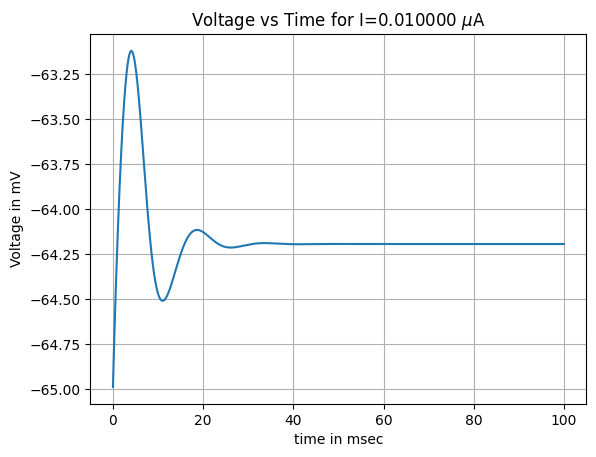
\includegraphics[width=0.6\textwidth]{./data/voltage_time_0_01uA.png}
    \caption{Plot of Voltage vs Time for I=0.01µA}
    \label{fig:voltage_time_0_01uA}
\end{figure}

\begin{figure}[H]
    \centering
    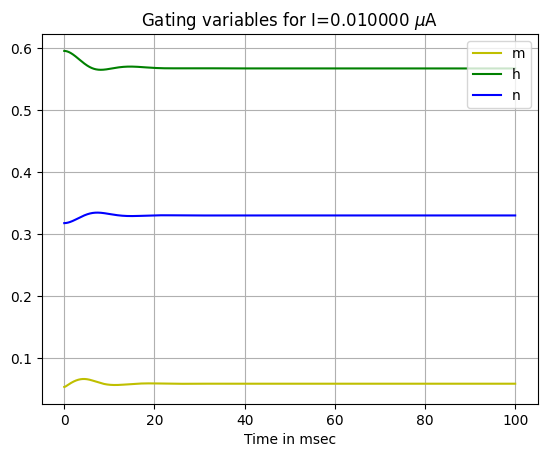
\includegraphics[width=0.6\textwidth]{./data/gating_variables_0_01uA.png}
    \caption{Plot of gating variables for I=0.01µA}
    \label{fig:gating_variables_0_01uA}
\end{figure}

\begin{figure}[H]
    \centering
    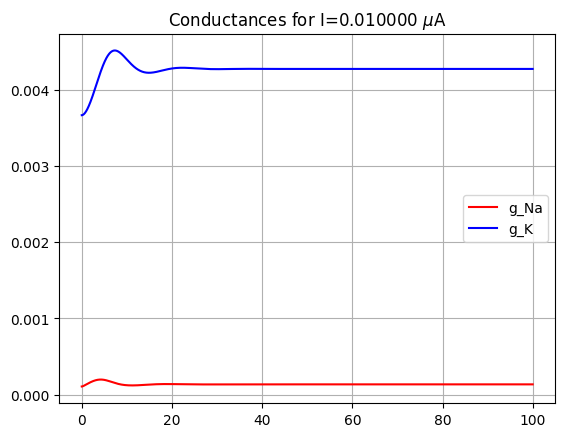
\includegraphics[width=0.6\textwidth]{./data/conductances_0_01uA.png}
    \caption{Plot of conductances for I=0.01µA}
    \label{fig:conductances_0_01uA}
\end{figure}



\begin{figure}[H]
    \centering
    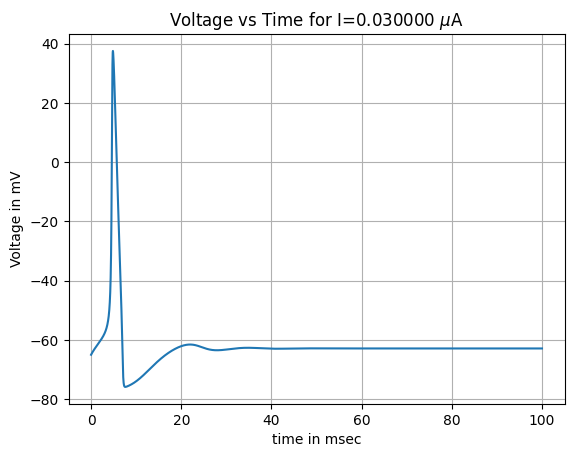
\includegraphics[width=0.6\textwidth]{./data/voltage_time_0_03uA.png}
    \caption{Plot of Voltage vs Time for I=0.03µA}
    \label{fig:voltage_time_0_03uA}
\end{figure}

\begin{figure}[H]
    \centering
    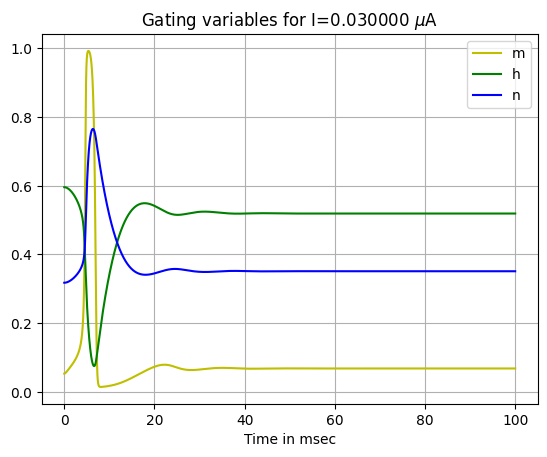
\includegraphics[width=0.6\textwidth]{./data/gating_variables_0_03uA.png}
    \caption{Plot of gating variables for I=0.03µA}
    \label{fig:gating_variables_0_03uA}
\end{figure}

\begin{figure}[H]
    \centering
    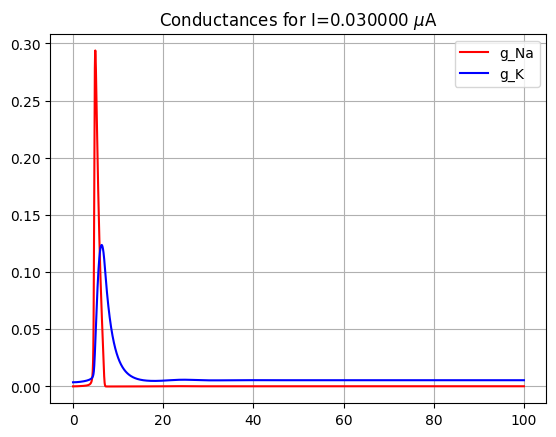
\includegraphics[width=0.6\textwidth]{./data/conductances_0_03uA.png}
    \caption{Plot of conductances for I=0.03µA}
    \label{fig:conductances_0_03uA}
\end{figure}



\begin{figure}[H]
    \centering
    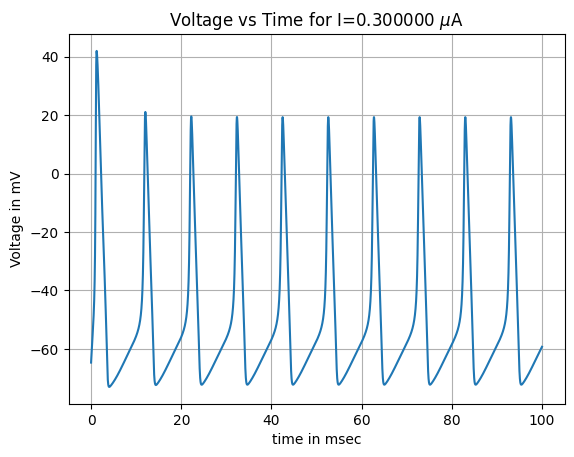
\includegraphics[width=0.6\textwidth]{./data/voltage_time_0_3uA.png}
    \caption{Plot of Voltage vs Time for I=0.3µA}
    \label{fig:voltage_time_0_3uA}
\end{figure}

\begin{figure}[H]
    \centering
    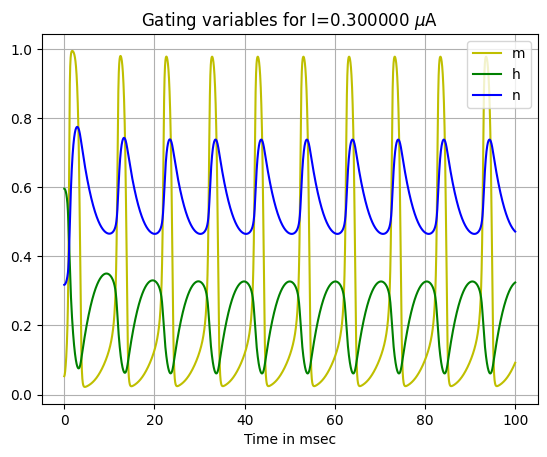
\includegraphics[width=0.6\textwidth]{./data/gating_variables_0_3uA.png}
    \caption{Plot of gating variables for I=0.3µA}
    \label{fig:gating_variables_0_3uA}
\end{figure}

\begin{figure}[H]
    \centering
    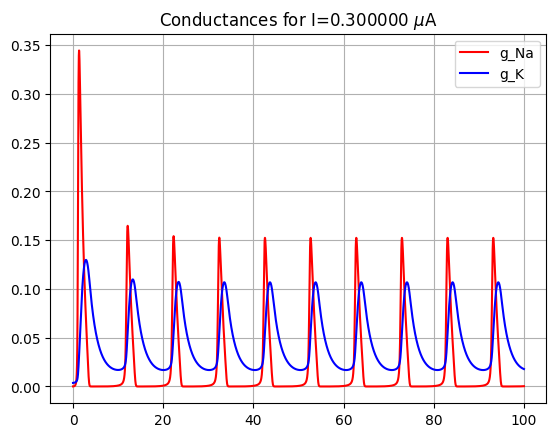
\includegraphics[width=0.6\textwidth]{./data/conductances_0_3uA.png}
    \caption{Plot of conductances for I=0.3µA}
    \label{fig:conductances_0_3uA}
\end{figure}

\begin{figure}[H]
    \centering
    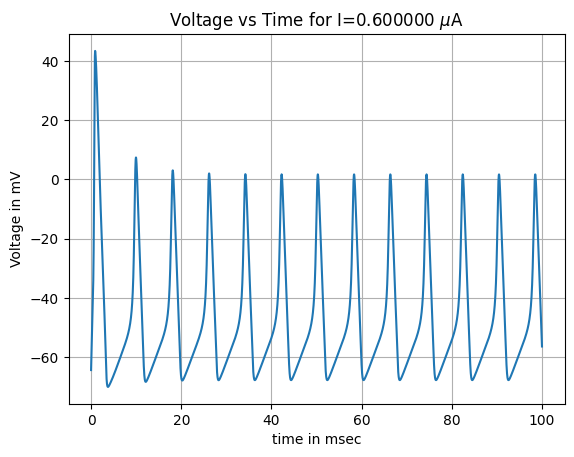
\includegraphics[width=0.6\textwidth]{./data/voltage_time_0_6uA.png}
    \caption{Plot of Voltage vs Time for I=0.6µA}
    \label{fig:voltage_time_0_6uA}
\end{figure}

\begin{figure}[H]
    \centering
    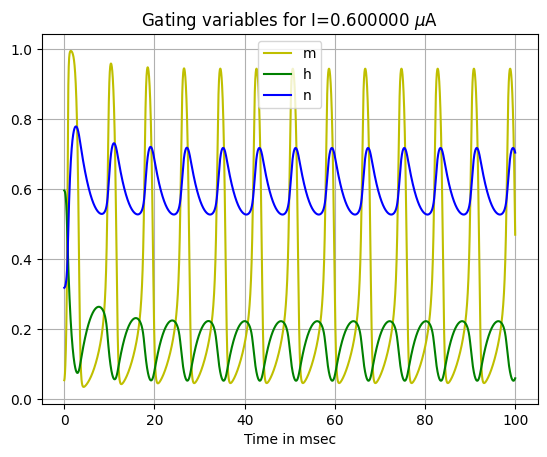
\includegraphics[width=0.6\textwidth]{./data/gating_variables_0_6uA.png}
    \caption{Plot of gating variables for I=0.6µA}
    \label{fig:gating_variables_0_6uA}
\end{figure}

\begin{figure}[H]
    \centering
    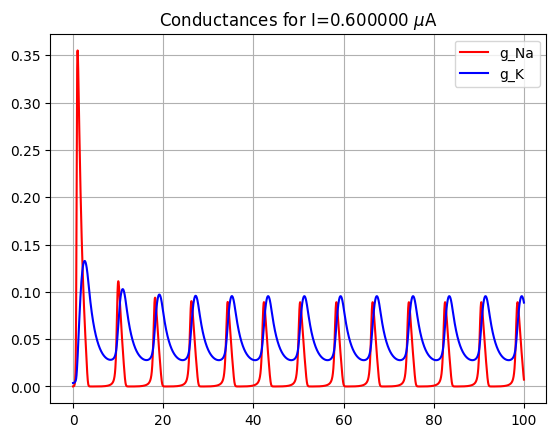
\includegraphics[width=0.6\textwidth]{./data/conductances_0_6uA.png}
    \caption{Plot of conductances for I=0.6µA}
    \label{fig:conductances_0_6uA}
\end{figure}


\chapter{Dynamics Of Neuron}

\section{Elements of Neuronal Systems}

Various types of neurons can be distinguished by the shape of their cell bodies and extensions. However, the network of neurons in the cortex is much more complex than what can be captured in a single picture. In fact, the cortex contains over \(10^{4}\) cell bodies and several kilometers of \textit{wires} per cubic millimeter, densely packed into a complex network that varies across different areas of the brain \cite{ref1}. Despite the differences in wiring patterns, all areas of the brain rely on neurons of different shapes and sizes as their building blocks. An example of such a neuronal network is depicted in Fig. 5.1, based on the early 20th century work of neuroscience pioneer Ramón y Cajal \cite{ref1}.

% Your figure code with the H specifier to force placement here
\begin{figure}[H]
\centering % Centers the figure
\fbox{% Adds a border to the figure
  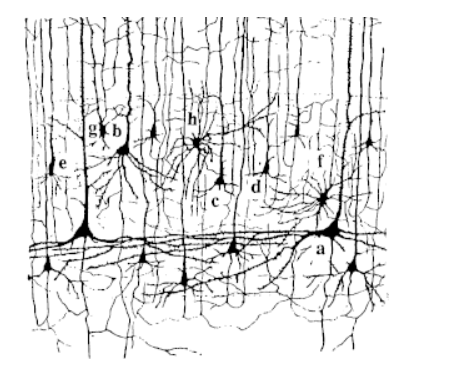
\includegraphics[width=0.8\textwidth]{./data/drawing.png} % Adjusts the size
}
\caption{A drawing of Ramón y Cajal showing a few neurons in the mammalian cortex \cite{ref2}} 
\end{figure}

The illustration reveals various neurons with distinct cell bodies and elongated projections, providing a snapshot of the densely woven neuronal networks in the cortex. In reality, the cortex’s neuronal networks are even more elaborate, with over 10,000 neuron cell bodies and extensive wiring in just one cubic millimeter. However, neurons are not the sole constituents of the cortex. It also comprises a multitude of glial cells, which play a supportive role in the brain’s energy management and structural integrity \cite{ref2}. 

When considering the physiology of neurons, it is important to note that their internal potential at rest is typically negative in comparison to their surroundings, often around -70mV. This negative resting potential is established by the combined action of various gating mechanisms, ion pumps, and ion channels present in the cell membrane \cite{ref3}. However, when the neuron's resting potential is perturbed beyond a certain level, such as due to input from other neurons, the ion channels in the membrane open and close in a coordinated manner to allow mainly ionic sodium and potassium (but also calcium and chloride) to pass through the membrane, resulting in a rapid and sharp change in potential. This sudden change generates a stereotyped pulse, or action potential, which travels along the axon of the neuron in an all-or-nothing manner, meaning that it is either fired with full amplitude or not fired at all.

The Hodgkin and Huxley model, developed over 50 years ago, provides a detailed description of a single neuron as a modified electrical circuit that transports electrical signals \cite{ref4}. This model explains how a single cell can regulate flows of ions through its cell membrane to rapidly depolarize and re-polarize itself, allowing for the generation of action potentials that become outputs to other neurons. In the human brain, which consists of approximately \(10^{11}\) neurons and \(10^{15}\) connections, neurons work as summing devices that sum up all their inputs, and depending on whether this sum reaches a certain threshold, respond by generating action potentials that become outputs to other neurons \cite{ref5}. These inputs may be either excitatory or inhibitory, resulting in an increase or decrease in the probability of the receiver neuron firing a response signal.

The brain processes information mainly by transmitting electric signals (action potentials) between millions of neurons across nerve fibers, with most modeling approaches considering only a subset of these. The fundamental questions in understanding the brain deal with how the activity of high numbers of interconnected neurons gives rise to a global activity pattern that is related to the function of the brain.


\begin{figure}[H]
    \centering % Centers the figure
    \fbox{% Adds a border to the figure
      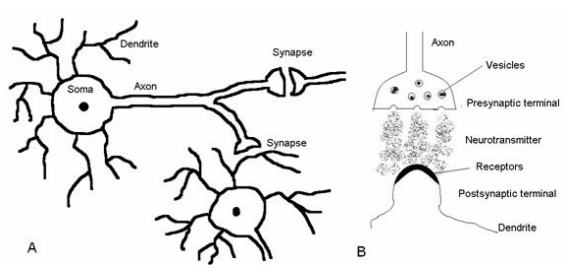
\includegraphics[width=0.8\textwidth]{./data/neuron.png} % Adjusts the size
    }
    \caption[A: A simple sketch of two neurons connected by a chemical synapse; B: A sketch of a chemical synapse]{\textbf{A:} A simple sketch of two neurons connected by a chemical synapse; \\ \textbf{B:} A sketch of a chemical synapse} 
\end{figure}
    
The brain adapts to environmental events and changes at three different time scales  \cite{ref6}. At the longest time scale, genetic adaptation results in a hard-wired connectivity of the neural network. At an intermediate time scale, the central nervous system adapts through numerous plastic mechanisms, forming assemblies of highly interacting and functionally associated neurons. Finally, at the shortest time scale, highly temporal changes in the neural activity are associated with the short-term states of the brain, which are closely related to cognitive processes \cite{ref7}.


\section{Neuron dynamics}
The human nervous system is composed of billions of individual nerve cells called neurons. Each neuron has a distinct structure that can be divided into segments such as the cell body, axon, and dendrites. The cell body contains the nucleus and other organelles that are essential for the neuron's proper functioning. The axon is a long, slender extension that carries electrical signals away from the cell body to other neurons or muscle cells. The dendrites are shorter, branched extensions that receive signals from other neurons and transmit them to the cell body. 

These different segments of the neuron work together to propagate action potentials, which are brief electrical impulses that allow neurons to communicate with one another. The interaction between the segments can be described as autonomous nonlinear systems, meaning that they operate independently and can exhibit complex, nonlinear behavior \cite{ref7}. These systems are crucial to the proper functioning of the nervous system, allowing us to perceive, process, and respond to the world around us.
\subsection{The Fitzhugh–Nagumo model}
The Fitzhugh-Nagumo model is a simplified mathematical representation of the neural dynamics of a neuron. It is essentially a third-order limit-cycle oscillator, which is characterized by the presence of two variables: the membrane potential V and the activation parameter n. The model exhibits different types of behavior depending on the control parameter a. Specifically, the system can display either stable fixed-point behavior or limit cycles. This model can shows table fixed-point behavior (Figs. 5.3(a) and (d)) or limit cycles (Figs. 5.3(c) and 3(d)), depending on the value of the control parameter. 


\begin{figure}[H]
    \centering % Centers the figure
    \fbox{% Adds a border to the figure
      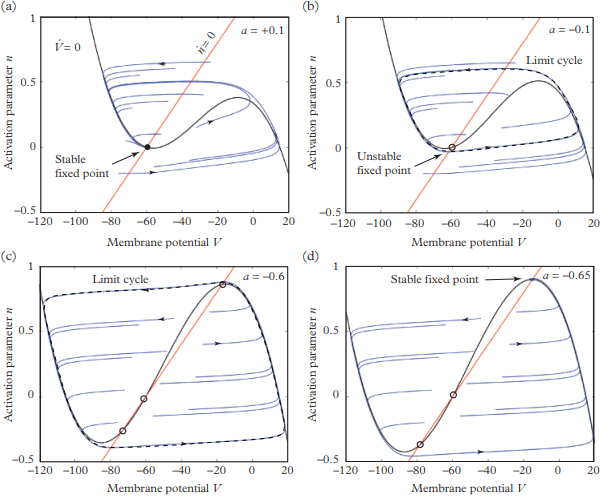
\includegraphics[width=0.8\textwidth]{./data/Fitzmodel.png} % Adjusts the size
    }
    \caption{Examples of the Fitzhugh–Nagumo model. The graph shows the membrane potential V on the horizontal axis and the activation parameter n on the vertical axis. The nullclines are plotted for n and V for I = 0. For a = +0.1, there is a stable fixed point in (a), while in (b) and (c) there are limit cycles representing neural spiking. In (d) for a = -0.67, the system converts back to a stable fixed point. \cite{ref8}} 
\end{figure}
    
When the stimulus is weak, the system is at a stable fixed point. In other words, it remains in a steady state, with the membrane potential and activation parameter both maintaining constant values. However, as the strength of the stimulus increases, the system undergoes a transition from resting potential to spiking. This means that the neuron starts to generate action potentials, which are brief but large electrical impulses that propagate along its axon and enable it to communicate with other neurons. The frequency and amplitude of these spikes can vary depending on the strength and duration of the stimulus\cite{ref8}. Overall, the Fitzhugh-Nagumo model provides a useful framework for understanding the basic mechanisms of neural activity and how they can be modulated by external inputs.
    
\subsection{The NaK model}
The NaK model is a sophisticated mathematical representation that illuminates the intricacies of two-dimensional phase planes. Its intriguing dynamics are contingent upon the bias current I, which can result in complex patterns of bistability and bifurcations. As a result, this model is highly useful for delving deeper into the parameter space and comprehending the diverse range of behaviors that it can exhibit. One of the interesting features of the NaK model is its ability to display bistability, which is an important aspect of neurodynamics. 

When a transient pulse is applied to the system, it can cause the system to cross the separatrix into the region where the dynamics relax onto the limit cycle. Once the system is on the limit cycle, it persists in a continuous oscillation. This type of behavior is characteristic of many biological systems, and the NaK model is a useful tool for studying and understanding these dynamics \cite{ref9}. The NaK model can display bifurcations as well as bistability. It allows a neuron to spike continuously even after the stimulus has been removed. 

When a short-lived pulse is introduced and then promptly withdrawn, it can elicit a response from the system that leads it to cross the separatrix and enter a state of sustained oscillation along a limit cycle \cite{ref10}. This phenomenon is illustrated in Fig. 5.4, and is observed in the NaK model when exposed to a current pulse of brief duration.


\begin{figure}[H]
    \centering % Centers the figure
    \fbox{% Adds a border to the figure
      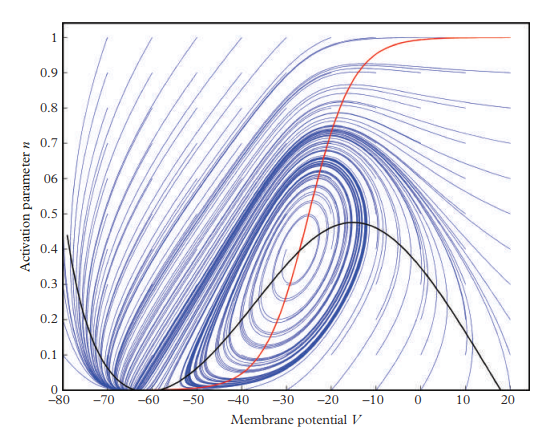
\includegraphics[width=0.8\textwidth]{./data/nak1.png} % Adjusts the size
    }
    \caption{Streamlines for the NaK model, show bistability\cite{ref9}} 
\end{figure}
    
    
Fig. 5.5 displays the phase diagram of the NaK model, which illustrates the situation where the stable node and the saddle point merge into a single saddle point. At this point, the limit cycle becomes a homoclinic orbit with an infinite period. This type of bifurcation is referred to as a saddle bifurcation, which can also be called a fold or a tangent bifurcation. In the NaK model, the harmonic orbit is connected to the saddle point.
    

\begin{figure}[H]
    \centering % Centers the figure
    \fbox{% Adds a border to the figure
      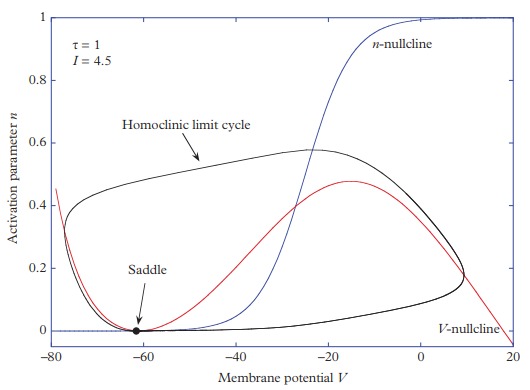
\includegraphics[width=0.8\textwidth]{./data/fig5.png} % Adjusts the size
    }
    \caption{A homoclinic orbit in the NaK model connected to the saddle point.\cite{ref9}} 
\end{figure}
    
Finally, the membrane potential for a trajectory close to the homoclinic orbit is demonstrated in Fig. 5.6. During the rapid traversal of the orbit, the membrane potential undergoes a quick change, and this is followed by a slow approach to the saddle point. This slow approach leads to a characteristic spiking appearance of the membrane potential. The spiking pattern is a result of the slow approach to the saddle, which causes the membrane potential to oscillate back and forth \cite{ref10}. These oscillations are responsible for the spiking appearance of the membrane potential.

\begin{figure}[H]
    \centering % Centers the figure
    \fbox{% Adds a border to the figure
      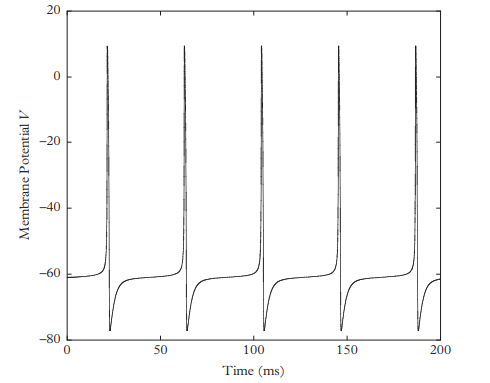
\includegraphics[width=0.8\textwidth]{./data/Fig6.png} % Adjusts the size
    }
    \caption{Membrane potential for an orbit near the homoclinic orbit as a time function.\cite{ref10}} 
\end{figure}



\chapter{Applications}
Biological neural network modeling is pushing the technological frontier in every field by simulating biological neural networks, solving real-world challenges, and improving the quality of human life. These applications demonstrate the power of interdisciplinary collaboration, bringing together biology, computer science, engineering and medicine to advance the future of medical technology and technology.

\begin{itemize}
    \item \textbf{ Brain-Computer Interface (BMI):} Brain-computer interface technology allows the human brain to interact directly with external devices, which has significant potential in providing assistive tools and restoring limb movement to paraplegic patients. Through the application of biological neural network models, researchers can better understand how brain signals map to body movements and how these signals can be interpreted to control external devices. These models also help improve algorithms to decode and translate brain activity into mechanical movements or electrical signals, enhancing the accuracy and responsiveness of brain-computer interfaces.
    \item \textbf{AI:} Biological neural networks provide artificial intelligence with a framework that mimics complex brain processing functions, particularly in the areas of vision and language processing. Deep learning, a biologically inspired algorithm, has led to breakthroughs in image recognition, speech-to-text conversion, and machine translation. Advances in these technologies, due in part to the understanding and simulation of how biological neural networks work, are changing the way we interact with technology and are finding applications in areas such as medicine, self-driving vehicles and smart homes.
    \item \textbf{Cognitive and Behavioral Research:} Biological neural network modeling helps scientists understand how cognitive processes are encoded in the brain. Such models can simulate memory formation, attention control, and decision-making processes, providing insights into studying behavior in humans and other animals. Additionally, they play an important role in explaining cognitive patterns in mental health conditions such as anxiety, depression, and other psychological disorders.
    \item \textbf{Precision medicine and disease diagnosis:} In the field of precision medicine, modeling of biological neural networks can predict how individuals will respond to specific treatments, thereby enabling personalized medicine. By analyzing a patient's gene expression data, protein levels and other biomarkers, the model is able to predict the course of the disease and the patient's response to drug treatment. Such models can also reveal new disease mechanisms, guide the development of future treatment strategies, and help physicians design customized treatment regimens to maximize efficacy and reduce side effects.
\end{itemize}


\chapter{Citations}
% \bibliographystyle{unsrt} % This specifies the style of the bibliography
% \bibliography{/Users/dengkai/workspace/papers/latex/config/ref} % This should match the name of your .bib file without the extension

\begin{thebibliography}{9}
    \bibitem{Mcculloch1854LOGICALCALCULUSIDEAS} Warren S Mcculloch and Walter Pitts. A LOGICAL CALCULUS OF THEIDEAS IMMANENT IN NERVOUS ACTIVITY. September 1854.
    \bibitem{Hebb2002OrganizationBehaviorNeuropsychological} D. O. Hebb. The Organization of Behavior: A Neuropsychological Theory. L.Erlbaum Associates, Mahwah, N.J, 2002.
    \bibitem{BernardWidrow1960AdaptiveSwitchingCircuits} Bernard Widrow and Marcian E. Hoff Jr. Adaptive Switching Circuits. 1960.
    \bibitem{Rosenblatt1958PerceptronProbabilisticModel} F. Rosenblatt. The perceptron: A probabilistic model for information storage and organization in the brain. Psychological Review, 65(6):386–408,1958.
    \bibitem{JJHopfield1982NeuralNetworksPhysical} J J Hopfield. Neural networks and physical systems with emergent collective computational abilities. April 1982.33
    
    \bibitem{Cole1939} Cole, K. S., Curtis, H. J. Electric impedance of the squid giant axon during activity. Journal of General Physiology, 22(5), 649–670 (1939). 
    \url{https://doi.org/10.1085/jgp.22.5.649}
    \bibitem{Hodgkin1939}HODGKIN, A., HUXLEY, A. Action Potentials Recorded from Inside a Nerve Fibre. Nature 144, 710–711 (1939).
    \url{https://doi.org/10.1038/144710a0}
    \bibitem{Hodgkin1949} Hodgkin, A. L., Katz, B. (1949). The effect of sodium ions on the electrical activity of the giant axon of the squid. The Journal of Physiology, 108. 
    \url{https://doi.org/10.1113/jphysiol.1949.sp004310}
    \bibitem{Hodgkin1952} Hodgkin, A. L., Huxley, A. F., (1952), A quantitative description of membrane current and its application to conduction and excitation in nerve. The Journal of Physiology, 117 
    \url{https://doi: 10.1113/jphysiol.1952.sp004764}
    \bibitem{Hausser2000} Häusser, M. The Hodgkin-Huxley theory of the action potential. Nat Neurosci 3 (Suppl 11), 1165 (2000). \url{https://doi.org/10.1038/81426}
    \bibitem{principles_of_neural_science}
    Kandel, E. R., Schwartz, J. H., Jessell, T. M., Siegelbaum, S. A., Hudspeth, A. J. (2014). Principles of Neural Science (5th ed.). McGraw-Hill Education. ISBN: 978-0-07-181001-2.


    \bibitem{ref1}
    S. Ramòn y Cajal (1909). \textit{Histologie du système nerveux de l’homme et des vertébrés}. A. Maloine, Paris.


    \bibitem{ref2}
    Ramón y Cajal S. (1894). The Croonian Lecture: La fine structure des centres nerveux. \textit{Proc. R. Soc. Lond.}, 55, 444--468.


    \bibitem{ref3}
    C. Cherniak, ``Local optimization of neuron arbors,'' \textit{Biol. Cybern.}, vol. 66, pp. 503--510, 1992.



    \bibitem{ref4}
    Hodgkin AL, Huxley AF (April 1952). ``Currents carried by sodium and potassium ions through the membrane of the giant axon of Loligo.'' \textit{The Journal of Physiology}, 116 (4): 449–472. 



    \bibitem{ref5}
    Chklovskii D.B., Mel B.W., Svoboda K. (2004). Cortical rewiring and information storage. \textit{Nature}, 431, 782--788.


    \bibitem{ref6}
    H. Reichert, \textit{Introduction to Neurobiology}. Oxford University Press, New York, 1992.


    \bibitem{ref7}
    G. Halnes, B. Fath, \& H. Liljenström (2007). The Modified Niche Model: Including Detritus in Simple Structural Food Web Models. \textit{Ecological Modelling}, 208, 9--16.

    \bibitem{ref8}
    H. Markram, M. Toledo-Rodriguez, Y. Wang, A. Gupta, G. Silberberg, \& C. Wu. 
    "Interneurons of the neocortical inhibitory system." \textit{Nature Reviews Neuroscience}, 5(10), 793-807, 2004.

    \bibitem{ref9}
    C. Wiedemann, M. Oswald, S. Stabroth, H. Klinkrad, P. Vörsmann, 
    ``Mathematical description of the NaK model for MASTER-2005,'' in \textit{Science Direct}, 2005.

    \bibitem{ref10}
    Bo Deng,
    ``Numerical Method for Homoclinic and Heteroclinic Orbits of Neuron Models,'' 
    \textit{Journal of Nonlinear Modeling and Analysis}, 
    vol. 1, no. 1, pp. 27–45, Mar. 2019, doi:10.12150/jnma.2019.27.
    
\end{thebibliography}





\chapter{Code}

\appendix


This code demonstrates the Hodgkin-Huxley model in current clamp experiments and shows action potential propagation.

\begin{lstlisting}[language=Python, caption={Python code for Hodgkin-Huxley simulation}, label={lst:python_code}]
#THIS PROGRAM DEMONSTRATES HODGKIN HUXLEY MODEL IN CURRENT CLAMP EXPERIMENTS AND SHOWS ACTION POTENTIAL PROPAGATION
#Time is in secs, voltage in mvs, conductances in m mho/mm^2, capacitance in uF/mm^2

# threshold value of current is 0.0223


import numpy as np
import matplotlib.pyplot as plt
from tqdm import tqdm
import sys
from numpy import NaN, Inf, arange, isscalar, asarray, array
ImpCur=0.6 #change input current here
g_K_max=.36 # max conductance of K channel
V_K=-77 #voltage of K channel
g_Na_max=1.20 #max conductance of Na channel
V_Na=50 #voltage of Na channel
g_l=0.003 #conductance of combined gates
V_l=-54.387 #voltageof combined channel
cm=.01

dt=0.01 #0.01 ms
niter=10000
t=np.array([i for i in range(niter)])
I_app=ImpCur*np.ones(niter)
V=-64.9964 #base voltage
m=0.0530
h=0.5960
n=0.3177


#### to store the values
g_Na_hist=np.zeros(niter)
g_K_hist=np.zeros(niter)
V_hist=np.zeros(niter)
m_hist=np.zeros(niter)
h_hist=np.zeros(niter)
n_hist=np.zeros(niter)

for i in range(niter):
    g_Na = g_Na_max*(m**3)*h
    g_K = g_K_max*(n**4)
    g_total = g_Na+g_K+g_l
    V_inf = ((g_Na*V_Na+g_K*V_K+g_l*V_l)+I_app[i])/g_total
    tau_v = cm/g_total
    V = V_inf+(V- V_inf)*np.exp(-dt/tau_v)
    alpha_m = 0.1*(V+40)/(1-np.exp(-(V+40)/10))
    beta_m = 4*np.exp(-0.0556*(V+65))
    alpha_n = 0.01*(V+55)/(1-np.exp(-(V+55)/10))
    beta_n = 0.125*np.exp(-(V+65)/80)
    alpha_h = 0.07*np.exp(-0.05*(V+65))
    beta_h = 1/(1+np.exp(-0.1*(V+35)))
    tau_m = 1/(alpha_m+beta_m)
    tau_h = 1/(alpha_h+beta_h)
    tau_n = 1/(alpha_n+beta_n)
    m_inf = alpha_m*tau_m
    h_inf = alpha_h*tau_h
    n_inf = alpha_n*tau_n
    m=m_inf+(m-m_inf)*np.exp(-dt/tau_m)
    h=h_inf+(h-h_inf)*np.exp(-dt/tau_h)
    n=n_inf+(n-n_inf)*np.exp(-dt/tau_n)
    V_hist[i]=V
    m_hist[i]=m
    h_hist[i]=h
    n_hist[i]=n

def plot_V_vs_t(V_hist,I_ext):
    plt.plot(t*dt,V_hist)
    plt.grid()
    plt.title('Voltage vs Time for I=%f $\mu$A'%I_ext)
    plt.xlabel('time in msec')
    plt.ylabel('Voltage in mV')
    plt.show()

def plot_gating_variables(m_hist,h_hist,n_hist,I_ext):
    plt.plot(t*dt,m_hist,'y',label='m')
    plt.plot(t*dt,h_hist,'g',label='h')
    plt.plot(t*dt,n_hist,'b',label='n')
    plt.xlabel('Time in msec')
    plt.title('Gating variables for I=%f $\mu$A'%I_ext)
    plt.grid()
    plt.legend()
    plt.show()

def plot_conductances(m_hist,h_hist,n_hist,I_ext):
    g_Na=g_Na_max*(m_hist**3)*h_hist
    g_K=g_K_max*n_hist**4
    plt.plot(t*dt,g_Na,'r',label='g_Na')
    plt.plot(t*dt,g_K,'b',label='g_K')
    plt.title('Conductances for I=%f $\mu$A'%I_ext)
    plt.legend()
    plt.grid()
    plt.show()
plot_V_vs_t(V_hist,ImpCur)
plot_gating_variables(m_hist,h_hist,n_hist,ImpCur)
plot_conductances(m_hist,h_hist,n_hist,ImpCur)

\end{lstlisting}





\end{document}


